\chapter{Data Understanding}

The dataset is composed by 10000 records. Each record represents a customer, described by $24$ different attributes.

\medskip

\section{Data semantics, distribution and statistics}

In this section we will analyze, for each attribute, its semantic and we will show interesting statistic and plot.
We have used two different colors for who went in credit default (green) and not (red) in order to better visualize their distribution among the different attributes.

We have discretized the continuous attributes by using the natural binning method. 

For these attributes the mode of the bin has also been reported as it is more representative.

%%%%%%%%%%%%%%%%%%%%%%%%%%%%%%%%%%%%%%%%%%%%%%%%%%%%%%
\smallskip
\begin{figure}[h]
  \begin{minipage}[h]{.50\textwidth}
        {\Large \textbf{Sex}}
        
        Gender of the customer.
        
        A binary attribute that can assume the values of \textit{male} ($3868$ of $10000$) or \textit{female} ($6032$ of $10000$). 
        
        Both of the gender values have a similar credit default rate ($25\%$ for males and $20\%$ for females).
  \end{minipage}
  \begin{minipage}[h]{.50\textwidth}
    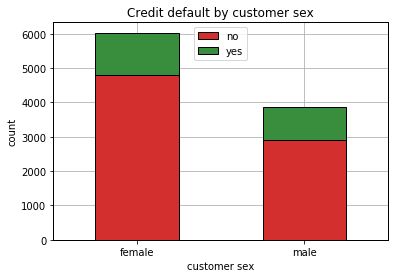
\includegraphics[width=.95\textwidth]{img/ch2/sex}
  \end{minipage}
\end{figure}

%%%%%%%%%%%%%%%%%%%%%%%%%%%%%%%%%%%%%%%%%%%%%%%%%%%%%%
\begin{figure}[h]
  \begin{minipage}[h]{.45\textwidth}
    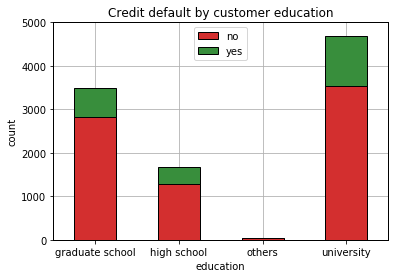
\includegraphics[width=.95\textwidth]{img/ch2/education}
  \end{minipage}
  \begin{minipage}[h]{.50\textwidth}
        {\Large \textbf{Education}}
        
        Qualification of the customer.
        
        A categorical attribute that can assume the values of 
        \textit{university} ($4685$ of $10000$),
        \textit{high school} ($1672$ of $10000$),
        \textit{graduate school} ($3480$ of $10000$) or
        \textit{others} ($36$ of $10000$).
        The default rate is again very similar for all the qualifications (around the $20\%$), except for the \textit{others} which is equal to $5\%$, but its number of records is very low to make any assumptions.
  \end{minipage}
\end{figure}

%%%%%%%%%%%%%%%%%%%%%%%%%%%%%%%%%%%%%%%%%%%%%%%%%%%%%%
\smallskip
\begin{figure}[h]
  \begin{minipage}[h]{.50\textwidth}
        {\Large \textbf{Status}}
        
        Marital status of the customer.
        
        A categorical attribute that can assume the values of 
        \textit{married} ($4685$ of $10000$),
        \textit{single} ($3757$ of $10000$) or
        \textit{other status} ($75$ of $10000$).
        
        The default rate is very similar for all the status (around the $25\%$).
  \end{minipage}
  \begin{minipage}[h]{.45\textwidth}
    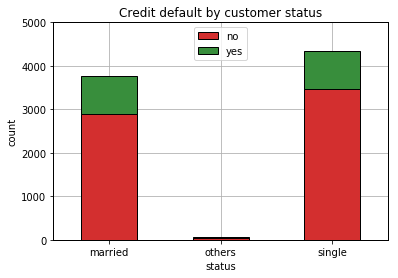
\includegraphics[width=.95\textwidth]{img/ch2/status}
  \end{minipage}
\end{figure}

%%%%%%%%%%%%%%%%%%%%%%%%%%%%%%%%%%%%%%%%%%%%%%%%%%%%%%
\smallskip
\begin{figure}[h]
  \begin{minipage}[h]{.45\textwidth}
    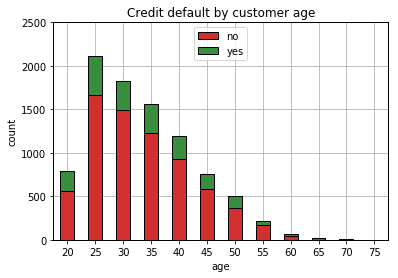
\includegraphics[width=.95\textwidth]{img/ch2/age}
  \end{minipage}
  \begin{minipage}[h]{.50\textwidth}
        {\Large \textbf{Age}}
        
        Age of the customer.
        
        An attribute that in the dataset assume integer values in $[21, 75]$, the lower limit to $21$ is due that in Taiwan the age of majority is $20$, on the other hand the upper limit can be as high as humanly possible.
        
        The average age is $35.49$, the standard deviation is $9.22$.
        The mode is $29$ and the median is $34$.
        The $50\%$ of the ages lie in $[28, 41]$.
        
        We decide to set a bin to $5$ year as it represent a good trade-off between the size and number of bins. The bin with most elements is $25$.
        
        Again the default rate is similar for all the bins (around $25\%$).
  \end{minipage}
\end{figure}

%%%%%%%%%%%%%%%%%%%%%%%%%%%%%%%%%%%%%%%%%%%%%%%%%%%%%%
\smallskip

\begin{figure}[h]
  \begin{minipage}[h]{.50\textwidth}
        {\Large \textbf{Limit}}
        
        Limit of the credit card (expressed in NT dollar).
        
        It is the maximum amount the credit card company will let borrow on the account, 
        a continuous attribute that can assume values in $[10000, 780000]$ (all values are multiples of $10000$).
        
        The average is $167197$ and the standard deviation is $128975$, $50\%$ of the ages lie in $[50000, 240000]$. The bin with most elements is $50000$.
        
        The default rate in this case is very different for each bin as it decrease with the limit: the first bin has a default rate of $38\%$, the second one of $26\%$ and around $10\%$ for the last bin.
        
  \end{minipage}
  \begin{minipage}[h]{.45\textwidth}
    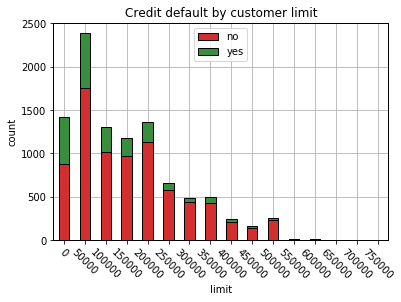
\includegraphics[width=.95\textwidth]{img/ch2/limit}
  \end{minipage}

\end{figure}

%%%%%%%%%%%%%%%%%%%%%%%%%%%%%%%%%%%%%%%%%%%%%%%%%%%%%%

\smallskip
\begin{figure}[h]
  \begin{minipage}[h]{.45\textwidth}
    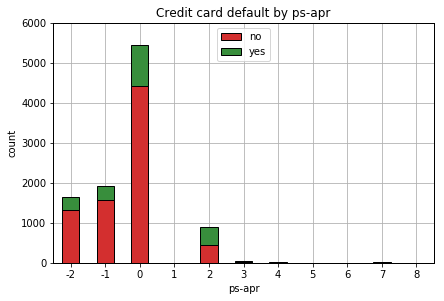
\includegraphics[width=.95\textwidth]{img/ch2/payment_status_1}
  \end{minipage}
  \begin{minipage}[h]{.55\textwidth}
        {\Large \textbf{Payment status}}
        
        History of past payments.
        
        Six categorical attributes that represent the repayment status, one for each month between April and September.
        A payment status is an integer number in the range $[-2, 9]$ where:
        
         $-2$ = no consumption
         
         $-1$ = paid in full
         
         $0$ = the use of revolving credit

         $1$ = payment delay for one month

         $2$ = payment delay for two months
         
         ...
         
         The distribution of the payment status over the six months are all very similar to each other so we only illustate the first one for simplicity.
         The most frequent bin is always the $0$ and around $90\%$ of the customers always lies between $-2$ and $0$. 
        
  \end{minipage}
\end{figure}

%%%%%%%%%%%%%%%%%%%%%%%%%%%%%%%%%%%%%%%%%%%%%%%%%%%%%%
\smallskip
\begin{figure}[h]
  \begin{minipage}[h]{.55\textwidth}
        {\Large \textbf{Bill Amount}}
        
        Amount of bill statement (expressed in NT dollar).
        
        Six continuous attributes, again one for each month between April and September.
        
        The bill amount is the sum of all the purchases, payments and other debits and credits made to your credit card account within the billing cycle. The values are in range $[-209051, 616836]$.
        As in the payment status, the distribution of the bill amount are nearly the same over the six month. The most frequent by is always the 0 (from $0$ NTD to $49999$ NTD).
        The mean increases according to the month, it start from $38621$ of April up to $51490$ of September. On ther other hand the credit default rate is always around the $20\%$ for all the bins (except some border case for small bin).
        
  \end{minipage}
  \begin{minipage}[h]{.45\textwidth}
    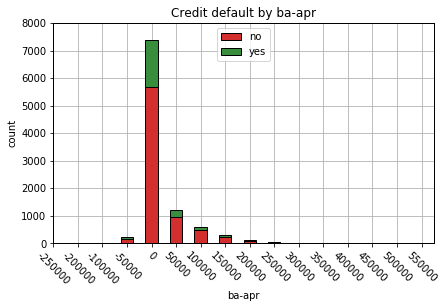
\includegraphics[width=.95\textwidth]{img/ch2/bill_amount_1}
  \end{minipage}
\end{figure}

%%%%%%%%%%%%%%%%%%%%%%%%%%%%%%%%%%%%%%%%%%%%%%%%%%%%%%
\smallskip
\begin{figure}[h]
  \begin{minipage}[h]{.45\textwidth}
    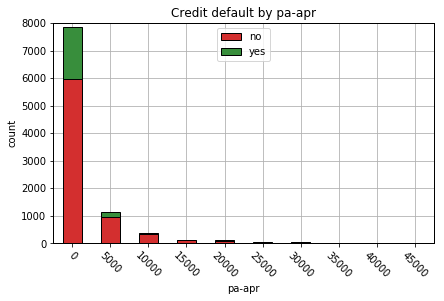
\includegraphics[width=.95\textwidth]{img/ch2/payment_amount_1}
  \end{minipage}
  \begin{minipage}[h]{.55\textwidth}
        {\Large \textbf{Payment amount}}
        
        Amount of payment (expressed in NT dollar).
        
        Six continuous attribute, one for each month between April and September.
        It represent the sum of all the payments made by the customer with the credit card in the last month. The distribution of the payment status over the six months are again all very similar to each other. The most frequent bin is always the 0 (from $0$ NTD to $4999$ NTD), which always include around the $75\%$ of the customers. The mean is around $4719$ and $5973$ without any particular distribution other the months.
  \end{minipage}
\end{figure}
%%%%%%%%%%%%%%%%%%%%%%%%%%%%%%%%%%%%%%%%%%%%%%%%%%%%%%
\smallskip
\begin{figure}[ht]
  \begin{minipage}[h]{.60\textwidth}
        {\Large \textbf{Credit default}}
        
        Credit card default.
        
        A boolean attribute that represents the credibility of the customer.
        The credit card default is a status that is applied to the customer when a list of terms are missed (like make the minimum required payment), and it affects for example your possibility to demand for a loan or to get another credit card. In the dataset we have $2212$ customer in credit card default and $7788$ not. 
        
  \end{minipage}
  \begin{minipage}[h]{.40\textwidth}
    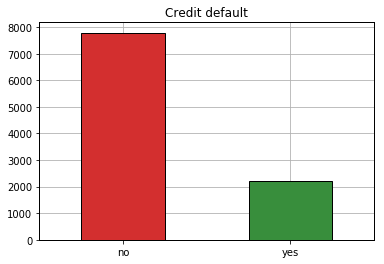
\includegraphics[width=.95\textwidth]{img/ch2/credit_default}
  \end{minipage}
\end{figure}

%%%%%%%%%%%%%%%%%%%%%%%%%%%%%%%%%%%%%%%%%%%%%%%%%%%%%%%%%%%%%%%%%%%%%%%%%%%%%%%
\clearpage

\section{Assessing data quality}

\begin{figure}[h]
  \begin{minipage}[h]{0.95\textwidth}

\begin{wrapfigure}{R}{0.40\textwidth}
\centering
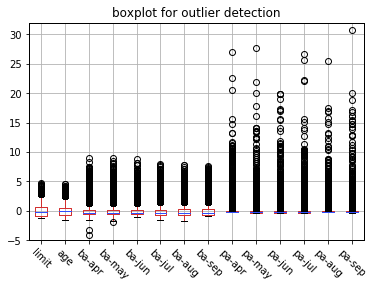
\includegraphics[width=0.40\textwidth]{img/ch2/outlier}
\end{wrapfigure}

    In this part we have checked for duplicates, missing values and outliers, in order to reduce the quantity of data and to avoid that their presence could negatively affect the analysis.

    Regarding the duplicates, in the dataset there are only two identical records so we decide to not remove the single duplicate as it is not a big problem.
    Regarding the missing values we have $100$ records with missing sex, $127$ records, $1822$ records with missing status and $951$ records with missing age. We decided to not remove them as they are a big part of the dataset, instead we replace the missing ages with the average age (which is $35.49$). We set the missing statuses to \textit{others} as we think that it can include some particular cases (like engaged or cohabitant). We again set the missing educations to \textit{others} and the missing sex to female as they are the more frequents in the dataset. 
    For the outliers we first normalize all the continuous attributes using the z-score algorithm (in this way we can visualize all the attributes in the same scale). Then we plot them in a boxplot and we can see that in the dataset only $3$ values are under the lower adjacent value, instead over the upper adjacent value we have $50$ limits, $211$ limits and an average of $895$ for the bill/payment amounts. We decided to not consider them outliers as we think that they represent the small percentage of rich people in the dataset (as they an high bill/payment amounts).
  \end{minipage}
\end{figure}

%%%%%%%%%%%%%%%%%%%%%%%%%%%%%%%%%%%%%%%%%%%%%%%%%%%%%%%%%%%%%%%%%%%%%%%%%%%%%%%
\section{Variables transformations}

We decide to transform the \textit{credit\_default} attribute from yes\/no to 1\/2 in order to better visualize them in the following plots. For the same reason and to limit the dispersion we decided to divide in bin the continuous attributes. In particular we divide ages in bin of $5$ years, payment amounts in bin of $1000$ NTD, limits and bill amounts in bin of $10000$ NTD.

As last transformation we have normalized all the continuous attribute using the min-max scaling.
%%%%%%%%%%%%%%%%%%%%%%%%%%%%%%%%%%%%%%%%%%%%%%%%%%%%%%%%%%%%%%%%%%%%%%%%%%%%%%%

\section{Correlations and redundant variables}

\begin{figure}[h]
  \begin{minipage}[h]{.95\textwidth}
  
    \begin{floatingfigure}[r]{0.55\textwidth}
        \mbox{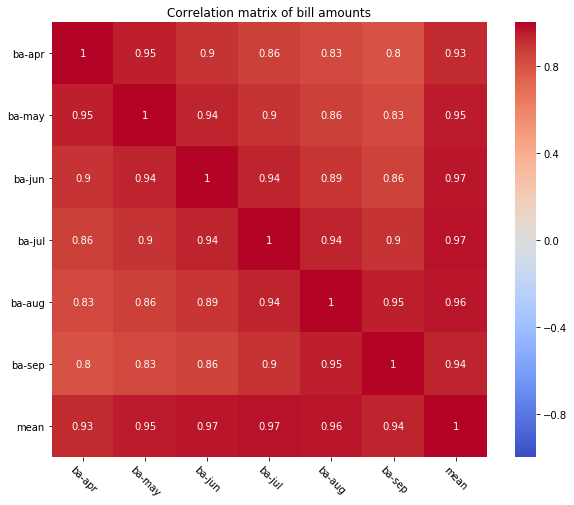
\includegraphics[width=0.55\textwidth]{img/ch2/correlation_matrix_ba}}
        \caption{correlation matrix with \textit{ba\_mean}}
    \end{floatingfigure}

  Analyzing the correlation matrix of all the continuous attribute we can clearly see that all the attributes related to the bill amounts are strongly correlated.

  All the pairs of bill amounts have a correlation between $0.8$ and $0.95$ so we decide to analize further this $6$ attributes.
    
  
  We added a new attribute to the dataset called \textit{ba\_mean} calculated as the mean of all the bill amount for each customer.
  
    
  We again plot the correlation matrix (rescricted only to the bill amounts attributes) and we can see that the mean has a correlation between $0.93$ and $0.97$. For this reasons we drop all the six bill amounts attributes and introduce \textit{ba\_mean} as new attribute. 


    
  \end{minipage}
\end{figure}
